\documentclass[a5paper]{article}

\usepackage{graphicx}
\usepackage{caption}
\usepackage{subcaption}
\usepackage{amsmath}
\usepackage{amsfonts}
\usepackage{amssymb}


\begin{document}
\setcounter{secnumdepth}{1}
\setcounter{tocdepth}{3}


	\begin{titlepage}
		\centering
		{\huge\bfseries Cantus Codex\par}
		\vspace{0.5cm}
        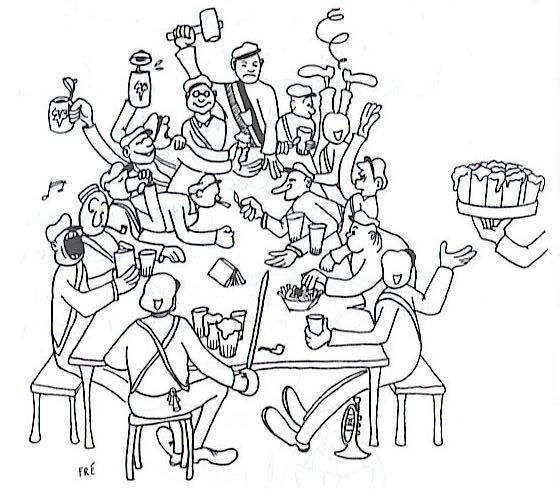
\includegraphics[height=6cm]{frontpicture.png}
		{\scshape\LARGE BEST Leuven\par}
		\vspace{0.5cm}
		
\includegraphics[height=1.5cm]{bestleuvenlogo.png}
		\vfill
		\vspace{0.5cm}
		{\scshape\LARGE Singer name: ..........................................\par}
	\end{titlepage}

	\tableofcontents

	\newpage



\section{The Rules}
\label{sec:rules}

A cantus is an old Belgian traditional night where students come together to sing and drink. This does not happen in a random way, everything is organized by a set of rules.

\subsection{Where it all starts…}
\label{sub:start}

The evening starts when the ``Senior'' enters the room. He will be the chairman or the big boss for tonight. The Senior opens the evening with the words $$\text{``CANTUS IN''},$$ which is Latin for: ``the cantus has started''. Traditionally, the first song has to be the ``Io Vivat'' and we sing this standing up with our right hand on our heart.

\subsection{Verbum} 
\label{sub:verbum}

Because a cantus is about tradition and respect, you should always address the senior in a formal way. If you want to say something in public you must stand up and ask the senior: $$\text{``SENIOR, PETO VERBUM''}.$$ The senior agrees: $$\text{``HABES''}$$ or refuses: $$\text{``NON HABES''}.$$


\subsection{Silentium} % (fold)
\label{sub:silentium}

% subsection silentium (end)

If the senior says: $$\text{``SILENTIUM''}$$ everybody must stop talking and obey the silence. 

\subsection{Standing and Sitting} % (fold)
\label{sub:standing_and_sitting}

% subsection standing_and_sitting (end)

The senior decides when you can sit by saying: $$\text{``OMNES AD SEDES''}.$$ You reply with $$\text{"SEDIMUS"}.$$ When you have to get up the senior says $$\text{``SURGITE''}$$ and you say $$\text{``SURGIMUS''}.$$ 

\subsection{Tempus} % (fold)
\label{sub:tempus}

If you want to leave the table (e.g. to go to the toilet), you must ask for it $$\text{``SENIOR, PETO TEMPUS''.}$$ The senior agrees: $$\text{``HABES''}$$ or refuses: $$\text{``NON HABES''.}$$ You might have to perform a little punishment or make a `pissing rhyme' in order to go to the toilet.

% subsection tempus (end)

\subsection{Singing} % (fold)
\label{sub:singing}

The senior will sometimes point somebody who has to sing the first lines of a song… Alone! After the first couple lines, the senior will say ``AD OMNES'' and then everybody sings along. If you don't know the song, please be silent and listen how to sing the song. Afterwards you can sing along.\\

We don't always sing the whole song. The senior indicates which strophe will be sung: 

\begin{table}[ht!]
\centering
\begin{tabular}{ l|r}
Latin & English \\
\hline
Ad Primam & The first \\
Ad Secundam & The second \\
Ad Tertiam & The third \\
Ad Ultimam & The last \\
\end{tabular}
\label{tab:stropheindicators}
\end{table}

% subsection singing (end)

\subsection{Drinking} % (fold)
\label{sub:drinking}

If you don't drink beer, you must mention this at the beginning of the evening. In this case another drink can be arranged.
Sometimes (actually a lot of times) the senior will instruct you to drink. He will do so in Latin. He will say or sing the words: $$\text{``PROSIT CORONA''.}$$ You must then answer with: $$\text{``PROSIT SENIOR''.}$$ The senior can say this as many times as he/she wants and you have to repeat it the same way. In the end the senior will give a drinking command:
$$\text{``AD FUNDUM''}$$ The whole glass in one time or $$\text{``AD LIBIDUM''}$$ Which means how much as you want.\\

When the senior commands you to drink, you always say the following \textbf{before} you drink: $$\text{PROSIT SENIOR, PROSIT CORONA}$$

For example the senior will say: $$\text{``PROSIT CORONA, AD FUNDUM''.}$$ So you will reply with: $$\text{PROSIT SENIOR, PROSIT CORONA,}$$$$\text{AD FUNDUM!.}$$ 
After that you drink your whole glass. \\

If you want to challenge somebody to drink you stand up \textbf{during a song} and say \textbf{quietly}: $$\text{``PROSIT, X''.}$$ If X accepts the challenge X then stands and responds: $$\text{"PROSIT, Y".}$$ And you both drink an Ad Fundum. Do not do this in the beginning of a cantus as you must survive the evening. It is not allowed to challenge the senior or to disturb the cantus.\\

Nobody can force you to drink. You can stop drinking beer and ask for water AT ANY TIME. Drinking is fun, but if you drink too much it is less fun for you, as well as for the others! You can always switch to water, it's not a sin, sometimes it's wise!

% subsection drinking (end)

\subsection{Punishments} % (fold)
\label{sub:punishments}

If the senior decides that you didn't obey him or broke one of the rules of the cantus, you will be asked to come to the middle. This is called $$\text{``AD PISTUM.''}$$ There you will have to perform a small and funny punishment, unless you were really bad!
% subsection punishments (end)

\newpage
\clearpage




\twocolumn
\section{Songs}
\label{sec:songs}

\subsection{Io Vivat} % (fold)
\label{sub:io_vivat}
Io vivat ! io vivat ! \\
Nostrorum sanitas !\\
Hoc est amoris poculum!\\
Doloris est antidotum !\\
Io vivat ! io vivat !\\
Nostrorum sanitas !\\
\\
Io vivat! io vivat!\\
Nostrorum sanitas !\\
Nos jungit amicitia,\\
Et vinum praebet gaudia.\\
Io vivat! io vivat!\\
Nostrorum sanitas !\\
\\
Io vivat ! io vivat !\\
Nostrorum sanitas !\\
Jam tota Academia,\\
Nobiscum amet gaudia.\\
Io vivat! io vivat!\\
Nostrorum sanitas !\\

\newpage
% subsection io_vivat (end)

\subsection{Gaudeamus Igitur} % (fold)
\label{sub:gaudeamus_igitur}

Gaudeamus igitur, Juvenes dum sumus; (bis)\\
Post icundum iuventutem,\\
Post molestam senectutem,\\
Nos habebit humus. (bis)	 \\
\\
Ubi sunt qui ante nos, In mundo fuere? (bis)\\
Vadite ad superos,\\
Transite ad inferos,\\
Ubi jam fuere. (bis)	 \\
\\
Pereat tristitia, Pereant osores, (bis)\\
Pereat diabolus,\\
Quivis antiburchius\\
Atque irrisores!	 (bis)\\

\newpage
% subsection gaudeamus_igitur (end)

\subsection{Clementine} % (fold)
\label{sub:clementine}

In a cavern, in a canyon,\\
Excavating for a mine,\\
Dwelt a miner, forty-niner, \\
and his daughter Clementine.\\
\\
\textit{Chorus:\\
\\
Oh my darling, Oh my darling, \\
Oh my darling Clementine ! \\
Thou art lost and gone forever, \\
Dreadful sorry, Clementine.}\\
\\
Light she was and like a fairy, \\
And her shoes were number nine; \\
Herring boxes, without topses, \\
Sandals were for Clementine.\\
\\
Drove she ducklings, to the water,\\
Every morning, just at nine;  \\
Hit her foot against a splinter,  \\
Fell into the foaming brine.\\
\\
Saw her lips above the water, \\
Blowing bubbles mighty fine, \\
But alas I was no swimmer \\
So I lost my Clementine.\\
\\
In my dreams she still doth haunt me, \\
Robed in garments soaked in brine, \\
While in life I used to hug her, \\
Now she's dead I draw the line.\\
\\
How I missed her, how I missed her, \\
How I missed my Clementine, \\
But I kissed her little sister, \\
And forgot my Clementine.\\

\subsection{Ein Prosit} % (fold)
\label{sub:ein_prosit}

Ein Prosit, ein Prosit \\
Der Gemütlichkeit \\
Ein Prosit, ein Prosit \\
Der Gemütlichkeit.\\

\newpage
% subsection clementine (end)

\subsection{Drunken Sailor} % (fold)
\label{sub:drunken_sailor}

% subsection drunken_sailor (end)

\begin{enumerate}
	\item What shall we do with the drunken sailor? (ter)\\
	Early in the morning?\\
	Hooray and up she rises, (ter)\\
	Early in the morning.\\
	\item Put him in the long-boat until he's sober.\\
	\item Pull out the plug and wet him all over.\\
	\item Put him in the scuppers with a hosepipe on him.\\
	\item Heave him by the leg in a running bowlin'.\\
	\item That's w'll do with the drunken sailor.\\
\end{enumerate}


% subsection ein_prosit (end)

\newpage

\subsection{Oh Susanna} % (fold)
\label{sub:oh_susanna}

I come from Alabama\\
With my banjo on my knee\\
I’m going to Louisiana\\
My true love for to see.\\
It rained all day the night I left\\
The weather was so dry\\
The sun so hot I froze myself\\
Susanna, don't you cry.\\
\\
\textit{Chorus:\\
\\
Oh! Sussana,\\
Oh! Don’t you cry for me;\\
For I come from Alabama\\
With my banjo on my knee.\\}
\\
I had a dream the other night,\\
When everything was still,\\
I thought I saw Susanna\\
A coming down the hill.\\
The buckwheat cake was in her mouth,\\
A tear was in her eye\\
I says, I'm coming from the South,\\
Susanna don't you cry.\\

\newpage
% subsection oh_susanna (end)

\subsection{Dis In Lucht} % (fold)
\label{sub:dis_in_lucht}


Foot on chair, foot on chair \\
Tralalalalire\\
Foot on chair, foot on chair \\
Tralalalala\\
\\
Two on chair, two on chair...\\
\\
Hand on table, hand on table... \\
\\
Table flies, table flies...\\
\\
Hand on glass, hand on glass...\\
\\
Glass to mouth, glass to mouth...\\
\\
Put glass down, put glass down...\\
\\
Table down, table down...\\
\\
Hand from table, hand from table...\\
\\
Foot off the chair, foot off the chair...\\
\\
Two off the chair, two off the chair...


% subsection dis_in_lucht (end)

\subsection{Auld Lang Syne} % (fold)
\label{sub:auld_lang_syne}

Should auld acquaintance be forgot,\\
And never brought to min’?\\
Should auld acquaintance be forgot,\\
And auld lang syne?\\
\\
\textit{Chorus:\\
\\
For auld lang syne, my dear,\\
For auld lang syne,\\
We'll take a cup o’ kindness yet,\\
For auld lang syne!\\}
\\
We twa hae run about the braes,\\
And pu'd the gowans fine,\\
But we've wander'd mony a weary foot,\\
Sin auld lang syne.\\
\\
We twa hae paidl'd i’ the burn\\
From morning sun till dine,\\
But seas between us braid hae roar'd\\
Sin auld lang syne.\\


\newpage
% subsection auld_lang_syne (end)

\subsection{Der Pappenheimer} % (fold)
\label{sub:der_pappenheimer}

Wir trinken einen Halben in der Welt. (bis)\\
Warum sollten wir nicht trinken einen Halben, (bis)\\
Einen Halben in der Welt.\\
General Pappenheimer 	)\\
Der soll leben 		)\\
General Pappenheimer 	)\\
Der lebe hoch. 		) bis\\
Bei Wein und bei Bier,\\
Lustige Pappenheimer sind wir hier;\\
Bei Wein und bei Bier,\\
Lustige Pappenheimer wollen \\wir sein.\\
\\
\textit{Replace ``in der Welt'' by:}\\
\\
... auf dem Stuhl.\\
... auf dem Tisch.\\
... unterm Tisch.\\
% subsection der_pappenheimer (end)

\newpage

\subsection{Chevalliers de la Table Ronde} % (fold)
\label{sub:chevalliers_de_la_table_ronde}

Chevaliers de la Table Ronde,       \\
Allons voir si le vin est bon.            \\
Allons voir oui oui oui,                   \\
Allons voir non non non, 	            \\
Allons voir si le vin est bon.          \\
\\
S'il est bon, s'il est agréable,\\
J'en boirais jusqu'a mon plaisir.\\
\\
J’en boirai cinq ou six bouteilles,\\
Une fille sur les genoux.\\
\\
Si je meurs, je veux qu'on m'enterre,\\
Dans la cave où y a du bon vin.\\
\\
Les deux pieds contre la muraille,\\
Et la tête sous le robinet!\\
\\
Sur ma tombe je veux qu'on inscrive,\\
``Ici g\^{i}t le Roi des Buveurs''! \\
\\
La morale de cette histoire,\\
C’est de boire avant de mourir.  \\

% subsection chevalliers_de_la_table_ronde (end)

\subsection{The Wild Rover} % (fold)
\label{sub:the_wild_rover}

I've been a wild rover \\
for many's a year,\\
I've spent all my money on \\
whiskey and beer,\\
But now I'm returning \\
with gold in great store,\\
And I never will play \\
the wild rover no more.\\
\\
\textit{Chorus:\\
\\
And it's no nay never, \\
no nay never no more,\\
Will I play the wild rover,\\
no never no more.\\}
\\
I went into an alehouse, \\
I used to frequent,\\
I told the landlady\\
my money was spent.\\
I asked her for credit, \\
she answered me nay.\\
Such custom like yours \\
I can have every day.\\
\\
I went up from my pockets\\
ten sovereigns bright,\\
And the landlady's eyes opened \\
wide with delight,\\
She says I have whiskeys \\
and wines of the best,\\
and the words that you told me\\
 were only in jest.\\
\\
I'll go home to my parents, \\
confess what I've done,\\
And I'll ask them to pardon \\
their prodigal son.\\
And when they've caressed me, \\
as oft times before,\\
Then I never will play \\
the wild rover no more. 

\newpage

% subsection the_wild_rover (end)

\end{document}